\documentclass[a4paper,14pt, unknownkeysallowed]{extreport}

\usepackage{cmap} % Улучшенный поиск русских слов в полученном pdf-файле
\usepackage[T2A]{fontenc} % Поддержка русских букв
\usepackage[utf8]{inputenc} % Кодировка utf8
\usepackage[english,russian]{babel} % Языки: русский, английский
\usepackage{enumitem}


\usepackage{threeparttable}

\usepackage[14pt]{extsizes}

\usepackage{caption}
\captionsetup{labelsep=endash}
\captionsetup[figure]{name={Рисунок}}

% \usepackage{ctable}
% \captionsetup[table]{justification=raggedleft,singlelinecheck=off}

\usepackage{amsmath}

\usepackage{geometry}
\geometry{left=30mm}
\geometry{right=15mm}
\geometry{top=20mm}
\geometry{bottom=20mm}

\usepackage{titlesec}
\titleformat{\section}
	{\normalsize\bfseries}
	{\thesection}
	{1em}{}
\titlespacing*{\chapter}{0pt}{-30pt}{8pt}
\titlespacing*{\section}{\parindent}{*4}{*4}
\titlespacing*{\subsection}{\parindent}{*4}{*4}

\usepackage{setspace}
\onehalfspacing % Полуторный интервал

\frenchspacing
\usepackage{indentfirst} % Красная строка
\setlength{\parindent}{1.25cm}

\usepackage{titlesec}
\titleformat{\chapter}{\LARGE\bfseries}{\thechapter}{20pt}{\LARGE\bfseries}
\titleformat{\section}{\Large\bfseries}{\thesection}{20pt}{\Large\bfseries}

\usepackage{multirow}
\usepackage{listings}
\usepackage{xcolor}

% Для листинга кода:
\lstset{ %
language=caml,                 % выбор языка для подсветки (здесь это С)
basicstyle=\small\sffamily, % размер и начертание шрифта для подсветки кода
numbers=left,               % где поставить нумерацию строк (слева\справа)
stepnumber=1,                   % размер шага между двумя номерами строк
numbersep=5pt,                % как далеко отстоят номера строк от подсвечиваемого кода
showspaces=false,            % показывать или нет пробелы специальными отступами
showstringspaces=false,      % показывать или нет пробелы в строках
showtabs=false,             % показывать или нет табуляцию в строках
frame=single,              % рисовать рамку вокруг кода
tabsize=2,                 % размер табуляции по умолчанию равен 2 пробелам
captionpos=t,              % позиция заголовка вверху [t] или внизу [b] 
breaklines=true,           % автоматически переносить строки (да\нет)
breakatwhitespace=false, % переносить строки только если есть пробел
escapeinside={\#*}{*)}   % если нужно добавить комментарии в коде
}



% plot
\usepackage{graphicx}
\usepackage{pgfplots}
\usepackage{filecontents}
\usetikzlibrary{datavisualization}
\usetikzlibrary{datavisualization.formats.functions}

\graphicspath{ {img/} }


\usepackage{subcaption}

\captionsetup{labelsep=endash}
\captionsetup[figure]{name={Рисунок}}



\usepackage[justification=centering]{caption} % Настройка подписей float объектов

\usepackage[unicode,pdftex]{hyperref} % Ссылки в pdf
\hypersetup{hidelinks}

\usepackage{csvsimple}

\newcommand{\code}[1]{\texttt{#1}}

\begin{document}
	
\begin{titlepage}
	\newgeometry{pdftex, left=2cm, right=2cm, top=2.5cm, bottom=2.5cm}
	\fontsize{12pt}{12pt}\selectfont
	\noindent \begin{minipage}{0.15\textwidth}
		
\includegraphics[width=\linewidth]{img/main_logo.jpg}
	\end{minipage}
	\noindent\begin{minipage}{0.9\textwidth}\centering
		\textbf{Министерство науки и высшего образования Российской Федерации}\\
		\textbf{Федеральное государственное бюджетное образовательное учреждение высшего образования}\\
		\textbf{«Московский государственный технический университет имени \newline Н. Э. Баумана}\\
		\textbf{(национальный исследовательский университет)»}\\
		\textbf{(МГТУ им. Н. Э.~Баумана)}
	\end{minipage}
	
	\noindent\rule{18cm}{3pt}
	\newline\newline
	\noindent ФАКУЛЬТЕТ $\underline{\text{«Информатика и системы управления»~~~~~~~~~~~~~~~~~~~~~~~~~~~~~~~~~~~~~~~~~~~~~~~~~~~~~~~}}$ \newline\newline
	\noindent КАФЕДРА $\underline{\text{«Программное обеспечение ЭВМ и информационные технологии»~~~~~~~~~~~~~~~~~~~~~~~}}$\newline\newline\newline\newline\newline\newline\newline
	
	
	\begin{center}
		\noindent\begin{minipage}{1.3\textwidth}\centering
		\Large\textbf{   ~~~ Лабораторная работа №4}\newline
		\textbf{по дисциплине "Анализ Алгоритмов"}\newline\newline\newline
		\end{minipage}
	\end{center}
	
	\noindent\textbf{Тема} 			$\underline{\text{Параллельные вычисления}}$\newline\newline
	\noindent\textbf{Студент} 		$\underline{\text{Светличная А.А.}}$\newline\newline
	\noindent\textbf{Группа} 		$\underline{\text{ИУ7-53Б}}$\newline\newline
	\noindent\textbf{Преподаватель} $\underline{\text{Волкова Л. Л., Строганов Ю.В.}}$\newline
	
	\begin{center}
		\vfill
		Москва~---~\the\year
		~г.
	\end{center}
	\restoregeometry
\end{titlepage}
	
	\setcounter{page}{2}
	\tableofcontents
	
\newpage
\chapter*{Введение}
	
\addcontentsline{toc}{chapter}{Введение}
	
Одной из главных задач программирования является ускорение решения вычислительных задач, которая может быть решена использованием параллельных вычислений.

В последовательном алгоритме решения какой-либо задачи есть операции, которые может выполнять только один процесс, например, операции ввода и вывода. 
Кроме того, в алгоритме могут быть операции, которые могут выполняться параллельно разными процессами. 
Способность центрального процессора или одного ядра в многоядерном процессоре одновременно выполнять несколько процессов или потоков, соответствующим образом поддерживаемых операционной системой, называют \textbf{многопоточностью} \cite{gladyshev}.

Процессом является программа в ходе своего выполнения. 
Каждый процесс состоит из одного или нескольких потоков - исполняемых сущностей, которые выполняют задачи, стоящие перед исполняемым приложением. 
После окончания выполнения всех потоков завершается процесс.

Современные процессоры могут выполнять две задачи на одном ядре при помощи дополнительного виртуального ядра. 
Такие процессоры называются многоядерными. 
Каждое ядро может выполнять только один поток за единицу времени. 
Если потоки выполняются последовательно, то их выполняет только одно ядро процессора, другие ядра не задействуются. 
Если независимые вычислительные задачи будут выполняться несколькими потоками параллельно, то будет задействовано несколько ядер процессора и решение задач ускорится.

	
\chapter{Аналитическая часть}
	
\section{Цель и задачи}
\textbf{Целью} данной лабораторной работы является изучение многопоточности на основе алгоритма Дейкстры (поиск кратчайших расстояний от одной вершины до всех остальных). 

Для достижения поставленной цели требуется выполнить следующие задачи:

\begin{itemize}
	\item изучить понятие параллельных вычилений;
	\item изучить последовательный и параллельный варианты алгоритма поиска кратчайших расстояний Дейкстры;
	\item реализовать изученные алгоритмы;
	\item провести сравнительный анализ по времени реализованных алгоритма;
	\item подготовить отчет о выполненной лабораторной работе.
\end{itemize}
	
	
\section{Алгоритм Дейкстры}

\textbf{Алгоритм Дейкстры} --- это последовательность действий, позволяющих оптимально найти на графе кратчайший путь от некоторой его вершины до всех остальных \cite{lebedev}.

Основная идея данного алгоритма заключается в том, что на каждом шаге помечается определённым образом выбранная вершина, а далее просматриваются все последующие (ещё не отмеченные) вершины графа и вычисляется длина пути до каждой из них от начальной
точки.
Помеченная на каждом этапе новая вершина (та, до которой путь оказался кратчайшим) становится определяющей для следующего шага. 
И этот построенный до неё кратчайший путь закрашивается.
Повторяя данные действия, последовательно просматривая и поочерёдно отмечая вершины графа, в итоге алгоритм добирается до конечного пункта. 
Те рёбра графа, которые в результате оказались закрашенными (вместе с отмеченными их крайними точками), образуют ориентированное дерево кратчайших путей (с корнем в исходной вершине графа). 
Далее остаётся выбрать на нём путь, который соединяет начальную точку с конечной. 
Это и будет искомый путь.

\section*{Вывод}
	
В данном разделе был изучен и рассмотрен алгоритм Дейкстры, хорошо подхлдящий для параллельных вычислений за счет того, что относительно каждого узла расматривает всех соседей независимо друг от друга.
	
\chapter{Конструкторская часть}

\section*{Описания алгоритмов}
\addcontentsline{toc}{section}{Описания алгоритмов}
	
На рисунке \ref{fig:dijkstra} представлены схема алгоритмов Дейкстры.

\begin{figure}[h!]
	\centering
	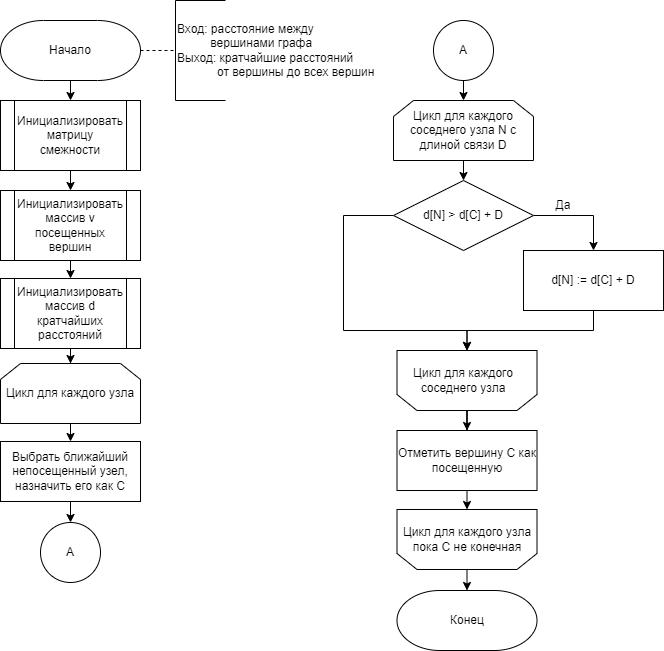
\includegraphics[width=0.95\linewidth]{img/dijkstra.png}
	\caption{Схема алгоритма Дейкстры}
	\label{fig:dijkstra}
\end{figure}

\section*{Вывод}
	
В данном разделе на основе теоретических данных были построены схема требуемого алгоритма.
	
\chapter{Технологическая часть}
	
\section{Требования к программному обеспечению}
	
В программе должна быть возможность:
	
\begin{enumerate}
	\item[1)] генирировать входные данные;
	\item[2)] находить кратчайшие расстояния от вершины одинм из указанных алгоритмов;
	\item[3)] замерять процессорное время выполнения реализаций алгоритмов.
\end{enumerate}
	
\section{Выбор языка программирования}
	
Для реализации алгоритмов поиска редакционных расстояний был выбран язык программирования С в силу наличия точных библиотек и быстродейственности языка.
	
\section{Выбор библиотеки и способа для замера времени}

Для замера процессорного времени выполнения реализаций агоритмов была выбрана не стандартная функция библиотеки <time.h> языка С~---~clock(), которая недостаточно четко работает при замерах небольших промежутков времени, а QueryPerformanceCounter - API-интерфейс, использующийся для получения меток времени с высоким разрешением или измерения интервалов времени.
        
Для облегчения работы с данным инструментом были самостоятельно написаны обертки-функции, представленные на листинге \ref{time}.
        
\clearpage
        
\begin{lstlisting}[label= time,caption=Функции замеров процессорного времени,language=C]
    LARGE_INTEGER frequency;
    LARGE_INTEGER t1,t2;
    double elapsedTime;

    void TIMER_INIT()
    {
        QueryPerformanceFrequency(&frequency);
    }
    
    void TIMER_START()
    {
    	QueryPerformanceCounter(&t1);
    }
    
    double TIMER_STOP()
    {
        QueryPerformanceCounter(&t2); 
        elapsedTime=(float)(t2.QuadPart-t1.QuadPart)/frequency.QuadPart/COUNT*MICRO;
    	
    	return elapsedTime;
    }

\end{lstlisting}
		
В силу существования явления вытеснения процессов из ядра, квантования процессорного времени все процессорное время не отдается какой-либо одной задаче, поэтому для получения точных результатов необходимо усреднить результаты вычислений: замерить совокупное время выполнения реализации алгоритма N раз и вычислить среднее время выполнения.
		
\section{Реализации алгоритмов}
	
В листингах \ref{dijkstra}, \ref{dijkstra_thread}, приведены реализации алгоритмов Дейкстры без использования параллельных вычислений и с использованием соответственно.

\clearpage

\begin{lstlisting}[label=dijkstra,caption=Алгоритм Дейкстры,language=C]
    void dijkstra(int a[SIZE][SIZE], int *d, int *v)
    {
        int temp, minindex, min;
        int begin_index = 0;
        
        d[begin_index] = 0;
      
        do {
            minindex = min = INT_MAX;
            for (int i = 0; i < SIZE; i++)
            {
                if ((v[i] == 1) && (d[i] < min))
                {
                    min = d[i];
                    minindex = i;
                }
            }
    
            if (minindex != INT_MAX)
            {
                for (int i = 0; i < SIZE; i++)
                if (a[minindex][i] > 0)
                    d[i] = get_min(2, d[i], min + a[minindex][i]);
                v[minindex] = 0;
            }
        } while (minindex < INT_MAX);
    }
\end{lstlisting}

\clearpage

\begin{lstlisting}[label=dijkstra_thread,caption=Алгоритм Дейкстры с использованием параллельных вычислений,language=C]
    typedef struct{
        int (*a)[SIZE];
        int* d;
        int min;
        int minindex;
        int i;
    } pthrData;


    void* threadFunc(void *thread_data)
    {
        pthrData *data = (pthrData*) thread_data;
	
        if (data->a[data->minindex][data->i] > 0)
            data->d[data->i] = get_min(2, data->d[data->i], 
            data->min + data->a[data->minindex][data->i]);
	
        return NULL;
    }

    void dijkstra_multi(int a[SIZE][SIZE], int *d, int *v)
    {
        pthread_t* threads = (pthread_t*) malloc(COUNT_THR * sizeof(pthread_t));
        pthrData* threadData = (pthrData*) malloc(COUNT_THR * sizeof(pthrData));

	
        int temp, minindex, min;
        int begin_index = 0;
    
        d[begin_index] = 0;
  
        do {
            minindex = min = INT_MAX;
            for (int i = 0; i < SIZE; i++)
            {
                if ((v[i] == 1) && (d[i] < min))
                {
                    min = d[i];
                    minindex = i;
                }
            }

            if (minindex != INT_MAX)
            {	
                for (int i = 0; i < SIZE; i += COUNT_THR)
                {		
                    for (int j = 0; j < COUNT_THR; j++)
                    {
                        threadData[j].a = a;
                        threadData[j].d = d;
                        threadData[j].min = min;
                        threadData[j].minindex = minindex;
                        threadData[j].i = i + j;
					
                        pthread_create(&(threads[j]), NULL, threadFunc, &threadData[j]);
                    }
                    for(int j = 0; j < COUNT_THR; j++)
                        pthread_join(threads[j], NULL);
                }
                v[minindex] = 0;
            }
        } while (minindex < INT_MAX);
    }
\end{lstlisting}

\section{Тестирование алгоритмов}

В таблице \ref{tbl:func_test} приведены функциональные тесты для функций, реализующих алгоритм Дейкстры. Все тесты пройдены успешно как алгоритмом без использования параллельных вычислений, так и алгоритмом с использованием.

\begin{table}[h]
    \captionsetup{justification=raggedright,singlelinecheck=off}
    \caption{\label{tbl:func_test} Функциональные тесты}
	\begin{center}
		\begin{tabular}{|c|c|}
			\hline
			Матрица A & Ожидаемый результат \\ 
			\hline
			$\begin{pmatrix}
				0
			\end{pmatrix}$ &
			0 \\
			\hline

			$\begin{pmatrix}
				0 & 37 \\
				37 & 0 \\
			\end{pmatrix}$ &
			0, 37 \\
			\hline
 
			$\begin{pmatrix}
                0 & 59 & 13 & 14 & 85 \\
                59 & 0 & 98 & 25 & 80 \\
                13 & 98 & 0 & 8 & 92 \\
                14 & 25 & 8 & 0 & 99 \\
                85 & 80 & 92 & 99 & 0 \\
			\end{pmatrix}$ &
			 0, 39, 13, 14, 85 \\
			\hline
   
		\end{tabular}
	\end{center}
	
\end{table}

\section*{Вывод}
В данном разделе были реализованы последовательный и параллельный алгоритма Дейкстры, а также проведено функциональное тестирование указанных алгоритмов.
	
\chapter{Экспериментальная часть}
	
\section{Технические характеристики}
Ниже приведены технические характеристики устройства, на котором было проведено тестирование программного обеспечения:
	
\begin{enumerate}
	\item[1)] операционная система Windows-10, 64-bit;
	\item[2)] оперативная память 8 ГБ;
	\item[3)] процессор	Intel(R) Core(TM) i3-7020U CPU @ 2.30GHz, 2304 МГц, ядер 2, логических процессоров 4.
\end{enumerate}
	
\section{Замеры времени}

В таблице \ref{table:t} приведены результаты замеров в микросекундах времени работы алгоритмов для входных графоф с разным количеством узлов.

\begin{table}[h!]
    \captionsetup{justification=raggedright,singlelinecheck=off}
    \caption{Замеры времени выполнения алгоритмов на произвольных массивах разной длины}
    \label{table:t}
	\begin{center}
        \begin{tabular}{| c | r@{.}l | r@{.}l | r@{.}l |}
        \hline
        Кол-во узлов &
        \multicolumn{2}{c|}{10} & 
        \multicolumn{2}{c|}{20} &
        \multicolumn{2}{c|}{50}\\ \hline
        
        1 & 2&98 & 8&67  & 48&36 \\ \hline 
				
        2 & 15475&22 & 59728&75 & 315804&90 \\ \hline 
		
        3 & 16409&54 & 58712&59 & 337089&45 \\ \hline 
				
        4 & 15970&94 & 51750&29 & 337464&52 \\ \hline 
				
        5 & 12853&70 & 51316&59 & 338854&04 \\ \hline
       
        \end{tabular}
    \end{center}
\end{table}

Из таблицы \ref{table:t} видно, что последовательный алгоритм работает намного быстрее, по этой причине стоит строить графики алгоритмов отдельно.

Зависимость времени работы последовательного алгоритма Дейкстры от количества узлов графа представлена на рисунке \ref{ris}.

\begin{center}
	\begin{figure}[h!]
	\center
	\begin{tikzpicture}
			\begin{axis} [
				legend pos = north west,
				grid = major,
				xmin = 10,
				ymin = 0, 
				xmax = 50,
				ymax = 50,
				xlabel = $\text{количество узлов}$,
				ylabel = $\text{время в мкс}$
				]
				\legend{ 
					$Onethread$, 
				};
				\addplot coordinates {
					(10, 2.98) (20, 8.67) (50, 48.36)
				};
			\end{axis}
	\end{tikzpicture}
	\caption{Зависимость времени работы последовательного алгоритма Дейкстры от количества узлов графа}
	\label{ris}
	\end{figure}
\end{center}

Из таблицы \ref{table:t} видно, что многопоточный алгоритм с разным количеством потоков работает за приблизительно одинаковое время, по этой причине строить все графики потоков нецелесообразно.

Зависимость времени работы многопоточного алгоритма Дейкстры от количества узлов графа представлена на рисунке \ref{ris}.

\begin{center}
	\begin{figure}[h!]
	\center
	\begin{tikzpicture}
			\begin{axis} [
				legend pos = north west,
				grid = major,
				xmin = 10,
				ymin = 15000, 
				xmax = 50,
				ymax = 350000,
				xlabel = $\text{количество узлов}$,
				ylabel = $\text{время в мкс}$
				]
				\legend{ 
					$2$,
                    $5$,
				};
				\addplot coordinates {
					(10, 15475.22) (20, 59728.75) (50, 315804.90)
				}; 
                \addplot coordinates {
					(10, 12853.70) (20, 51316.59) (50, 338854.04)
				};
			\end{axis}
	\end{tikzpicture}
	\caption{Зависимость времени работы многопоточного алгоритма Дейкстры от количества узлов графа}
	\label{ris}
	\end{figure}
\end{center}
	
\section*{Вывод}
	
В данном разделе былпа проведена оценка эффективности реализаций последовательного и многопоточного алгоритма Дейкстры, которая показала, что последовательный алгоритм выигрывает в скорости, это происходит по причине того, что выбранная для распараллеливания операция является слишком маленькой относительно всего алгоритма, а для выполнения каждой такой операции в многопоточном режиме необходимо сохранить большое количество данных, что и увеличивает время работы данной реализации.
	
\chapter*{Заключение}

\addcontentsline{toc}{chapter}{Заключение}

\textbf{Цель} данной лабораторной работы достигнута --- изучена многопоточность на основе алгоритма Дейкстры. 

Все \textbf{задачи} выполнены:

\begin{itemize}
	\item изучено понятие параллельных вычилений;
	\item изучены последовательный и параллельный варианты алгоритма поиска кратчайших расстояний Дейкстры;
	\item реализованы изученные алгоритмы;
	\item проведен сравнительный анализ по времени реализованных алгоритма;
	\item подготовлен отчет о выполненной лабораторной работе.
\end{itemize}
	
На основании проведенных экспериментов было определено, что быстродействие работы последователього алгоритма Дейкстры много больше параллельного варианта данного алгоритма, что происходит по причине незначительности параллельной операции в соотношении с необходимыми для многопоточности действиями.
	
\addcontentsline{toc}{chapter}{Список использованных источников}

\nocite{*} 

\renewcommand\bibname{Список использованных источников} % переименовать страницу списка литературы
\bibliographystyle{utf8gost705u}  % стилевой файл для оформления по ГОСТу
\bibliography{lib}          % имя библиографической базы (bib-файла)
	
\end{document}
